\section{Bitcoin}
\label{sec:bitcoin}
Bitcoin (codice: BTC o XBT) è una criptovaluta e un sistema di pagamento mondiale creato nel 2009 da un anonimo inventore, noto con lo pseudonimo di Satoshi Nakamoto, che sviluppò un'idea da lui stesso presentata su Internet a fine 2008. Per convenzione se il termine Bitcoin è utilizzato con l'iniziale maiuscola si riferisce alla tecnologia e alla rete, mentre se minuscola (bitcoin) si riferisce alla valuta in sé.\cite{wiki-bitcoin}
\\Il progetto Bitcoin è nato con l'intento di risolvere i problemi di fiducia, trasparenza e responsabilità tra due parti nello scambio di denaro per beni e servizi su Internet, senza l’utilizzo di intermediari. Bitcoin, infatti, rappresenta la prima rete di pagamento che utilizza una tecnologia distribuita peer-to-peer per operare senza un'autorità centrale: la gestione delle transazioni e l'emissione di denaro sono effettuati collettivamente dalla rete.
\\La rete Bitcoin utilizzando la tecnologia blockchain, è una catena di blocchi concatenati tra di loro, infatti ogni blocco contiene il riferimento al hash del blocco precedente. Questo sistema è immutabile perchè se si volesse modificare un blocco si dovrebbero modificare tutti i blocchi successivi ad esso, per fare ciò si dovrebbe creare una catena di blocchi che è più lunga di quella esistente. Ovviamente, la distribuzione e la natura delle tempistiche del processo rendono praticamente impossibile che ciò accada.
\\Inotre, utilizzando un sistema distribuito, permette di tenere traccia di tutti i trasferimenti in modo da evitare il problema del double spending (spendere due volte). Tutti gli utenti sono a conoscenza di ciò che accade e pertanto non c’è bisogno di una autorità centrale che gestisca le transazioni.
\\In aggiunta, Bitcoin consente il possesso e il trasferimento anonimo delle monete, ed infatti i dati necessari per usufruire dei propri bitcoin sono salvati in uno o più personal computer sotto forma di digital wallet (portafoglio). I bitcoin sono trasferiti tramite Internet a chiunque disponga di un indirizzo bitcoin. La struttura peer-to-peer della rete e l’assenza di un ente centrale rende impossibile a qualsiasi autorità il blocco dei trasferimenti, il sequestro dei bitcoin senza il possesso delle relative chiavi o la svalutazione dovuta all’immissione di nuova moneta. Per questo motivo i bitcoin sono la moneta più utilizzata nel Deep Web.
\\
\\Ricapitolando, le principali caratteristiche su cui si basa questo sistema di enorme successo sono le seguenti:
\begin{itemize}
\item \textbf{Nessuna autorità centrale}: non dipende da nessuna terza parte privata o ente governativo, e, pertanto, il valore dei BTC è liberamente contrattato sul mercato. Si tratta quindi di un sistema decentralizzato;
\item \textbf{Irreversibile e non falsificabile}: una volta che una transazione è stata effettuata ed è inclusa nella blockchain, non può più essere annullata, nemmeno dal mittente;
\item \textbf{Anonimo}: chiunque può scaricare il software ed iniziare ad effettuare transazioni, senza registrarsi, senza comunicare dati personali e senza svelare la propria identità.
\item \textbf{Sistema distribuito su rete Peer-to-peer (rete paritaria o paritetica)}: qualsiasi nodo è in grado di avviare e completare una transazione in modo autonomo.
\item \textbf{Inflazione determinata a priori}: L’emissione di nuovi BTC è determinata dall’algoritmo stesso del programma, e non può essere modificata.
\end{itemize}
Per capire meglio questi punti, verrà illustrata in modo dettagliato una transazione tra due utenti Alice e Bob che vogliono scambiarsi bitcoin.

\begin{figure}[H]
	\centering
	
\includegraphics[width=0.3\textwidth]{images/bitcoinLogo.png}
	\caption{Logo Bitcoin.}
	\label{fig:bitcoinLogo}
\end{figure}

\subsection{Come avviene una transazione}
\label{sec:come avviene una transazione}
Un esepio pratico di scambio di moneta aiuterà nel capire come funziona il sistema. I nostri attori saranno Alice (pagante) e Bob (ricevente).
\\
\\I passi da eseguire sono:
\begin{enumerate}\itemsep2pt

\item Bob comanda alla sua applicazione (wallet) su PC o smartphone di creare un indirizzo. Il software restituisce una sequenza alfanumerica da 26 a 35 caratteri. Questo è un esempio: 12gXGyXWkvyDAjVKZHyGGstVYyXJ6ZjgqV

\item Bob copia l'indirizzo e lo mostra al mittente tramite qualunque mezzo: via mail, messaggio, QR code, pubblicato su un sito internet, scritto su carta, dettato al telefono etc.

\item Alice inserisce nel suo software l'indirizzo di Bob e la quantità di Bitcoin da inviare, inoltre specifica l'ammontare della commissione da pagare al minatore (detto "miner") per convalidare la transazione. Ad oggi i più comuni software stabiliscono automaticamente una commisione fissa a 0,00001 bitcoin.

\item Bob vede immediatamente sul suo software la transazione avvenuta, ma prima di considerare il pagamento effettuato attende che la transazione sia inserita nella blockchain.

\item In un massimo di 10 minuti circa la transazione viene inserita in un blocco della blockchain da parte del miner, che ha convenienza a inserirla perché in questo modo ottiene la commissione pagata da Alice.

\item Bob può sentirsi sicuro che la transazione è confermata con l’aumentare di blocchi che vengono aggiunti alla blockchain conseguentemente a quello che contiene la transazione. 

\item Bob avrà nel proprio portafoglio i bitcoin inviati da Alice per spenderli in una nuova transazione.
\end{enumerate}

\begin{figure}[H]
	\centering
	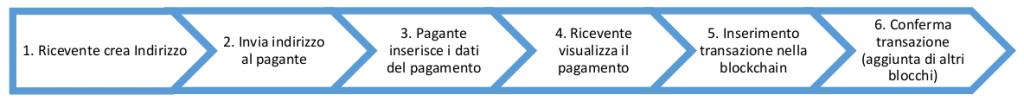
\includegraphics[width=\textwidth]{images/transazioneBitcoin.png}
	\caption{Come avviene una transazione Bitcoin.}
	\label{fig:bitcoinTransaction}
\end{figure}

\subsection{Come avviene una transazione dal punto di vista tecnico}
\label{sec:come avviene una transazione dal punto di vista tecnico}
La stessa transazione affrontata con un occhio più tecnico, soffermando l'attenzione sulla parte di creazione delle chiavi e della conferma ed aggiunta del blocco.
\\
\\I passi da eseguire sono:
\begin{enumerate}\itemsep2pt
\item Tramite il software che si occupa del wallet, Bob genera in modo del tutto casuale una chiave privata, che viene salvata sul suo computer.
\item La chiave privata viene convertita in una chiave pubblica tramite un procedimento matematico. Comunemente è il software di Bob a generare automaticamente la chiavi quando Bob chiede all'applicazione di creare un indirizzo da comunicare al mittente. In realtà Bob potrebbe utilizzare una chiave privata facilmente ricordabile, come “sum qui sum”, e ricavare Public key e indirizzo da questa. Il procedimento matematico si basa su un algoritmo chiamato “Elliptic Curve Digital Signature Algorithm”\cite{bitcoin:ECDSA} che utilizza la curva ellittica.
\\È teoricamente possibile ma statisticamente impraticabile scoprire la chiave privata partendo da quella pubblica: poiché il procedimento matematico applicato è unidirezionale, il processo inverso per indovinare la chiave privata richiederebbe una quantità di tentativi e una potenza di calcolo talmente enorme da essere al di là di ogni possibilità
\item La chiave pubblica viene a sua volta crittografata e accorciata tramite un hash. Possiamo chiamare la nuova chiave pubblica Public Key Hash. La chiave pubblica originaria invece è detta Full Public Key.
\item L'hash della chiave pubblica viene convertito in una riga di massimo 35 caratteri (per comodità pratica), che costituisce l'indirizzo del portafoglio di Bob. Per esempio: 12gXGyXWkvyDAjVKZHyGGstVYyXJ6ZjgqV.
\item Bob spedisce l'indirizzo ad Alice.
\begin{figure}[H]
	\centering
	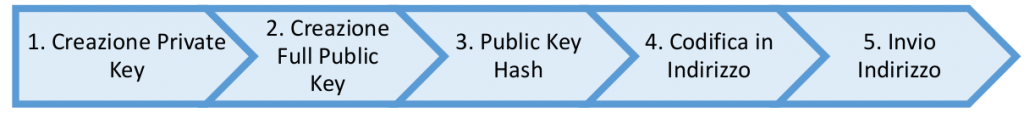
\includegraphics[width=\textwidth]{images/passiDiBob.png}
	\caption{Azioni del ricevente.}
	\label{fig:bobSteps}
\end{figure}
\item Il software di Alice decodifica immediatamente l'indirizzo in una normale Public Key Hash
\item \label{aliceCreaTransazione} Alice crea la transazione. Si può pensare la transazione come un codice che contiene diverse informazioni, ciascuna rappresentabile come una stringa composta da molti caratteri:
\begin{itemize}
	\item l’input: uno o più output di una transazione precedente fatta nei confronti 	di Alice, da cui ella attinge i bitcoin che «spedisce» nel nuovo output
	\item l'output: la quantità di bitcoin spediti. Possono esserci più output per 			ogni transazione, ciascuno identificato con un ID specifico
	\item l'istruzione per la firma (la "signature script"): ovvero le le istruzioni 		che Bob dovrà fornire per convalidare la transazione, dimostrando di essere il 			possessore del nuovo output. È proprio per la creazione dello script che il 			software di Alice ha bisogno del Public Key Hash fornito da Bob. Le informazioni 		necessarie per validare la firma sono due, entrambe già in possesso di Bob: la 			full Public Key e la Private Key, che dovranno combaciare col Public Key Hash 			specificato da Alice nello script.
\end{itemize}
Queste informazioni vengono processate insieme nella creazione di un unico hash chiamato txid (transaction identifier)
\begin{figure}[H]
	\centering
	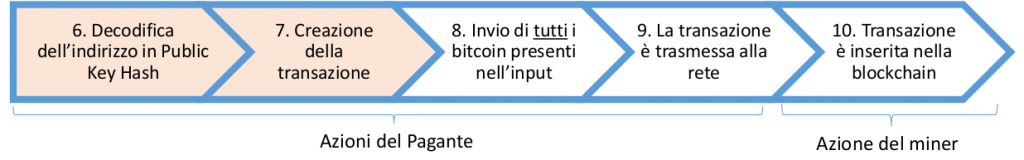
\includegraphics[width=\textwidth]{images/passiAlice1.png}
	\caption{Prima parte. Azioni del pagante.}
	\label{fig:aliceSteps1}
\end{figure}
\item Tutti i bitcoin che Alice ha a disposizione su un particolare input vengono "spediti" nella transazione. Infatti nella transazione è coinvolta sempre l'intera quantità di bitcoin presenti nell’input anche se Bob ne ha richiesti molti meno. Se Alice dispone di un input di 100 bitcoin e ne trasferisce 20 a Bob, l’input è sempre trasferito nella sua interezza di 100 bitcoin. In questo caso avrà due output diversi, uno di 80 bitcoin (al lordo della commissione per il miner) che tornano al portafoglio di Alice (il change output), l'altro di 20 bitcoin che vanno all'indirizzo di Bob. L’unico caso di transazione che abbia un solo input e un solo output è quello in cui l’input corrisponde esattamente all’ammontare richiesto da chi riceve i bitcoin. Spesso le transazioni hanno più output, e quindi i bitcoin trasferiti vanno ad indirizzi con diverse chiavi pubbliche e private.
\item Alice trasmette via internet al software di tutti gli altri nodi tutte le informazioni relative alla transazione. I nodi sono rappresentati da tutti coloro che hanno il software Bitcoin Core sui propri pc/dispositivi o numerosi altri software che permettono di "collegarsi" al network Bitcoin.
\begin{figure}[H]
	\centering
	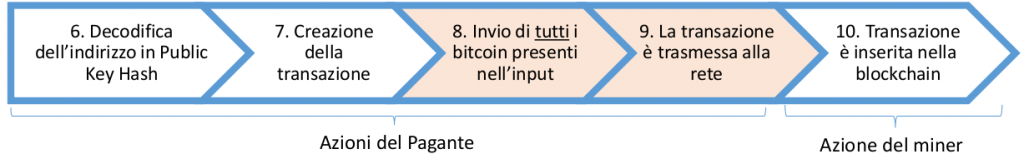
\includegraphics[width=\textwidth]{images/passiAlice2.png}
	\caption{Seconda parte. Azioni del pagante.}
	\label{fig:aliceSteps2}
\end{figure}

\item I minatori inseriscono le transazioni ancora non confermate nella blockchain.
\\Per inserire le transazioni all’interno della blockchain il miner deve creare un nuovo blocco, processo che richiede una quantità di calcolo molto elevata e dunque una spesa in energia elettrica e strumenti. Un miner ha interesse a inserire quante più transazioni nel blocco che vuole creare poiché guadagnerà tutte le commissioni pagate su ciascuna transazione. Se una transazione non include alcuna commissione, il miner non ha alcun interesse economico nell’inserirla nel blocco.

\begin{figure}[H]
	\centering
	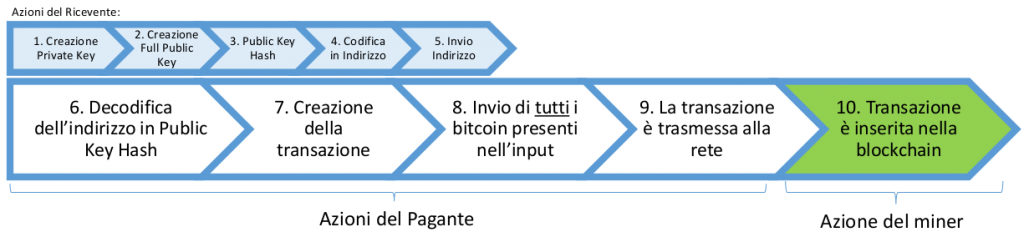
\includegraphics[width=\textwidth]{images/azioneMiner.png}
	\caption{Azione dei miner.}
	\label{fig:minerSteps}
\end{figure}

Per inserire le transazioni nel blocco, i minatori partono dagli id delle transazioni (txid), ciascuno dei quali rappresenta l’hash di tutte le informazioni inerenti una singola transazione (passo \ref{aliceCreaTransazione}).
\\I txid sono accoppiati due a due, creando un hash per ogni coppia di transazioni. Ogni hash viene poi accoppiato con un altro hash, creando un hash figlio dei due hash precedenti, e così via finché non si arriva a un unico hash. In caso di numeri dispari un hash viene processato con una sua copia identica. Questo procedimento può essere rappresentato come un albero, il cosiddetto Merkle tree [\ref{fig:merkelTree}],  dove le foglie sono le transazioni txid, i rami (biforcuti) gli hash intermedi e la radice l’hash finale, prodotto di tutti gli altri hash: la Merkle root. L’hash finale è come l’ultimo di una stirpe e porta con sé il “DNA” di tutti gli hash precedenti\cite{merkle-tree}.
\\Grazie alla struttura del Merkle tree, non è necessario conoscere tutte le transazioni incluse in un blocco per verificare che una singola transazione ne faccia parte, è invece sufficiente seguire un particolare ramo che collega una foglia (una transazione) alla merkle root.
\begin{figure}[H]
	\centering
	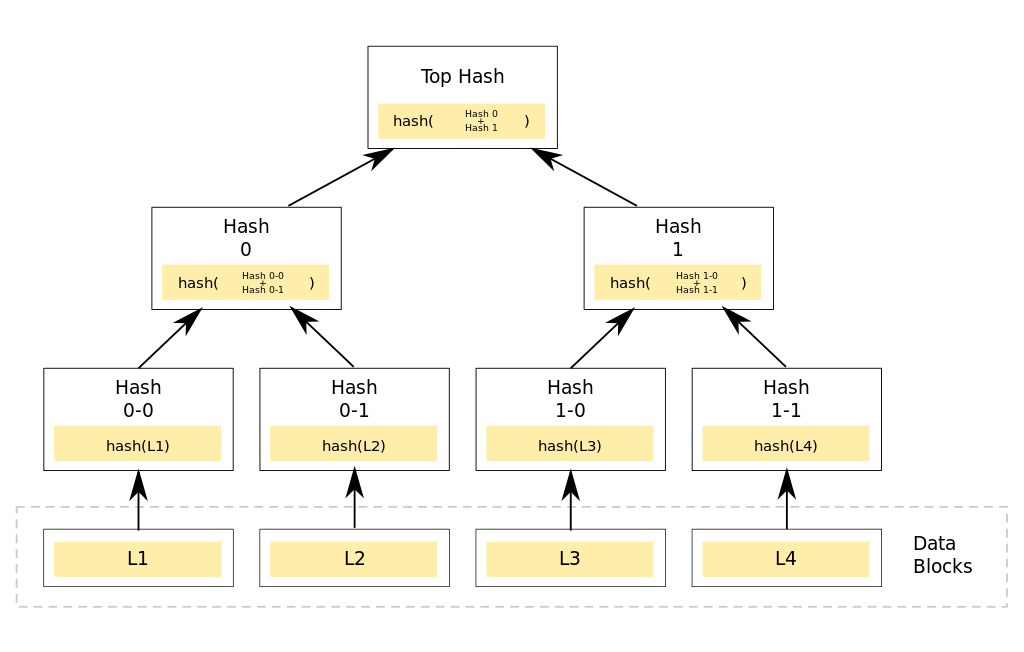
\includegraphics[width=\textwidth]{images/merkle_tree.png}
	\caption{Merkle tree.}
	\label{fig:merkelTree}
\end{figure}

\item Bob ora vuole spendere i suoi nuovi bitcoin in una nuova transazione, il destinatario è Charlie. Bob segue la stessa procedura che ha seguito Alice, creando una transazione specificando output, signature script (per cui gli serve il public key hash di Charlie), timestamp e versione del software.
\\Bob però deve dimostrare di essere il possessore dei bitcoin che invia a Charlie, ovvero i bitcoin presenti nell’input della transazione. Tale input è anche l’output della transazione fra Alice e Bob. Quest’ultimo per dimostrare di possedere l’ouput di quella transazione deve porre la sua firma (signature). Bob inserisce quindi la sua Full Public Key, verificando che corrisponde al Public Key Hash dato in precedenza ad Alice, e la sua Private Key, che rappresenta la conferma che Bob solo è la persona che ha originato inizialmente quella Public Key. Infatti seppur sia teoricamente possibile, è per motivi statistici «infattibile» scoprire la Private Key partendo dalla Public Key. Il procedimento di firma è del tutto automatizzato dal software Bitcoin\cite{transazioneBitcoin}.

\end{enumerate}